% Propósito: derivar visualmente la ley del cuadrado inverso a partir del área
% de dos superficies esféricas atravesadas por la misma potencia.
% Origen: S=4 pi r^2 e I=W/S, ecuaciones
% \eqref{eq:u4-cuadrado-inverso} y
% \eqref{eq:u4-razon-intensidades-distancia}. La relación de presión requiere
% además las condiciones declaradas antes de
% \eqref{eq:u4-nivel-presion-distancia}.
% Esquema geométrico en sección; no está a escala ni representa una fuente real.
% Descripción accesible: dos circunferencias concéntricas representan secciones
% de esferas de radios r y 2r alrededor de una fuente. La esfera exterior tiene
% cuatro veces el área. Como ambas son atravesadas por la misma potencia, la
% intensidad exterior es un cuarto y, en campo lejano progresivo, la presión
% eficaz es la mitad.
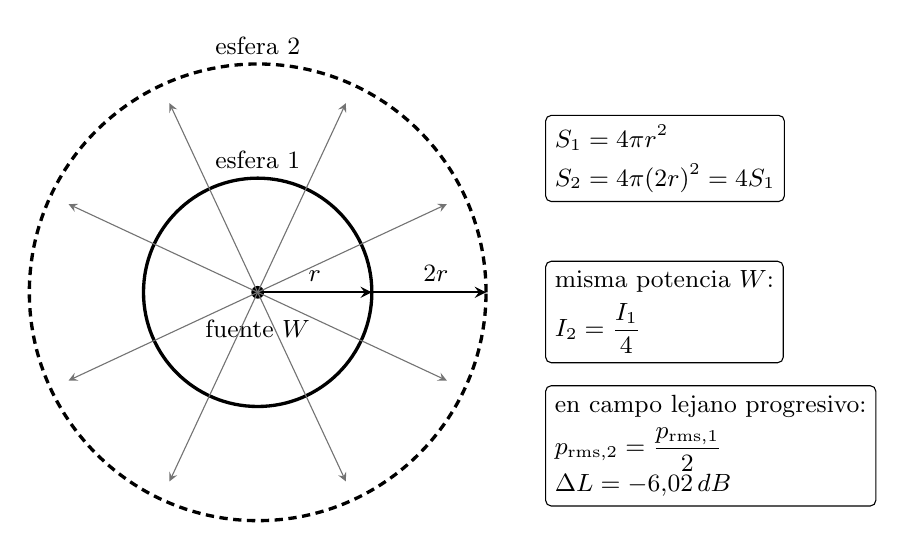
\begin{tikzpicture}[font=\small,>=stealth,x=1cm,y=1cm]
    \coordinate (S) at (3.35,3.20);
    \fill (S) circle (2.3pt);
    \node[below,fill=white,inner sep=1.5pt] at ([yshift=-3mm]S)
        {fuente \(W\)};

    \draw[very thick] (S) circle (1.45cm);
    \draw[very thick,densely dashed] (S) circle (2.90cm);
    \node[above] at (3.35,4.65) {esfera 1};
    \node[above] at (3.35,6.10) {esfera 2};

    \draw[->,thick] (S) -- (4.80,3.20)
        node[midway,above] {\(r\)};
    \draw[->,thick] (S) -- (6.25,3.20)
        node[pos=0.78,above] {\(2r\)};

    \foreach \a in {25,65,115,155,205,245,295,335}{
        \draw[->,black!55] (S) -- ++(\a:2.65);
    }

    \node[draw,rounded corners=2pt,align=left,anchor=west] at (7.00,4.90)
        {\(\displaystyle S_1=4\pi r^2\)\\[3pt]
         \(\displaystyle S_2=4\pi(2r)^2=4S_1\)};
    \node[draw,rounded corners=2pt,align=left,anchor=west] at (7.00,2.95)
        {misma potencia \(W\):\\[3pt]
         \(\displaystyle I_2=\frac{I_1}{4}\)};
    \node[draw,rounded corners=2pt,align=left,anchor=west] at (7.00,1.25)
        {en campo lejano progresivo:\\[3pt]
         \(\displaystyle p_{\mathrm{rms},2}
            =\frac{p_{\mathrm{rms},1}}{2}\)\\
         \(\displaystyle \Delta L=-6{,}02\,\text{dB}\)};
\end{tikzpicture}
